\documentclass[cheatsheet.tex]{subfiles}
\begin{document}
A classifier is a mapping that maps instances to classes. $\hat{c}(x)$ is an estimate of the (presumably) true but unknown function c(x) (aka the oracle). The training data comprises labeled instances. 
\subsection{Binary Classification}
Two-class classification (k = 2, binary classification) is known as concept learning. 
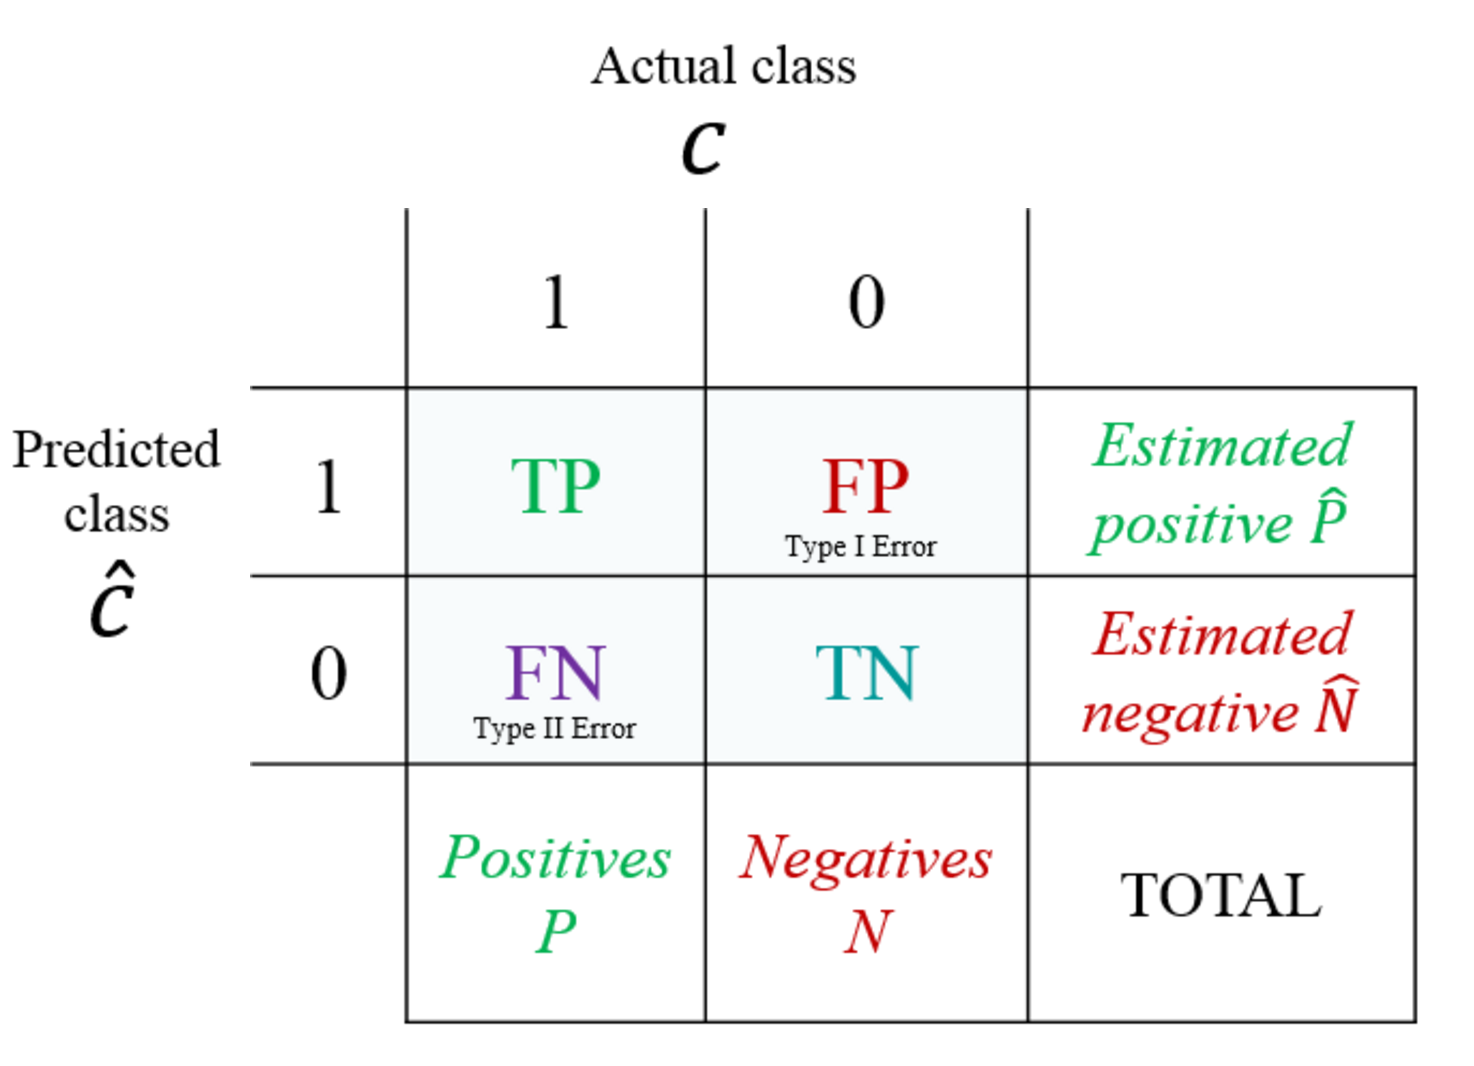
\includegraphics[width=40mm]{contingency_table.png}
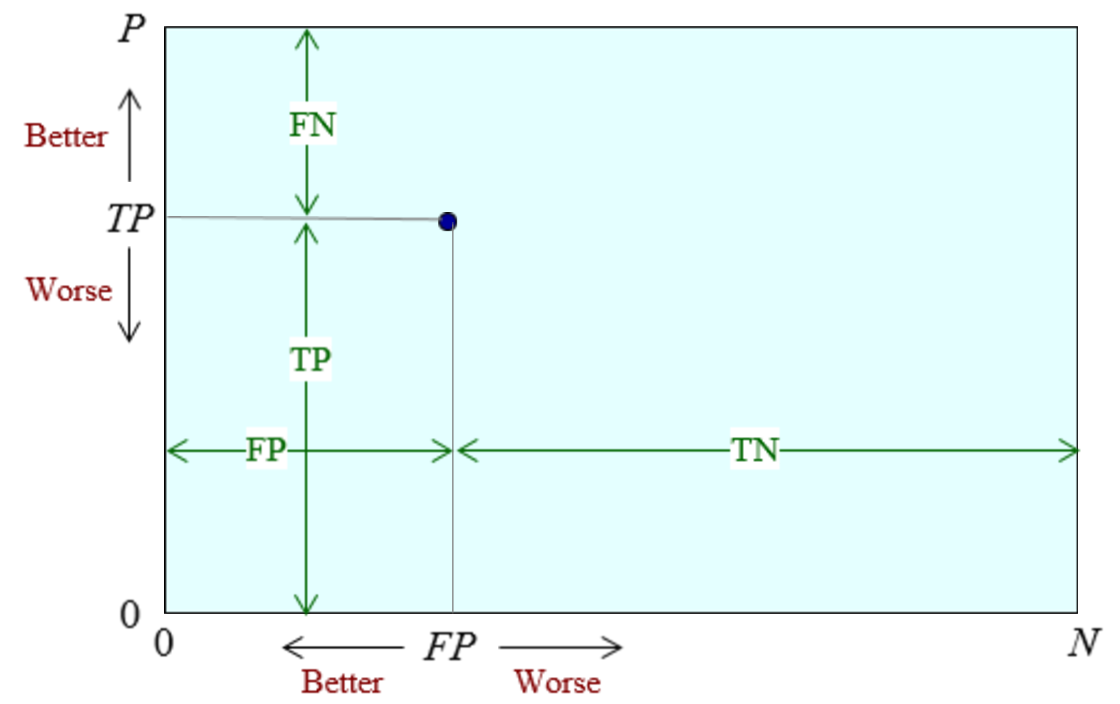
\includegraphics[width=40mm]{coverage_plot.png}
\\
In a coverage plot, classifiers with the same accuracy are connected by line segments with slope 1. In an ROC plot, line segments with slope 1 connect classifiers with the same average recall. 
\subsection{Scoring \& Ranking}
A scoring classifier is a mapping, along with a class decision based on the scores (typically
highest score). We can turn the feature tree into a scoring tree by computing a
score for each leaf: 
\textbf{Score:} $\hat{s}(x)=log_2 \frac{spam}{ham}$\\
\textbf{Margin:} $z(x)=c(x)\hat{s}(x)$, \textbullet Positive if the estimate $\hat{s}(x)$ is correct, Negative if $\hat{s}(x)$ is incorrect. \textbullet Large positive margins mean "strongly correct", Large negative margins mean "the classifier screwed up".
\\
In learning a classifier, we'd like to reward large positive margins and penalize large negative margins by the use of a loss function that maps the margin to an associated loss. \\
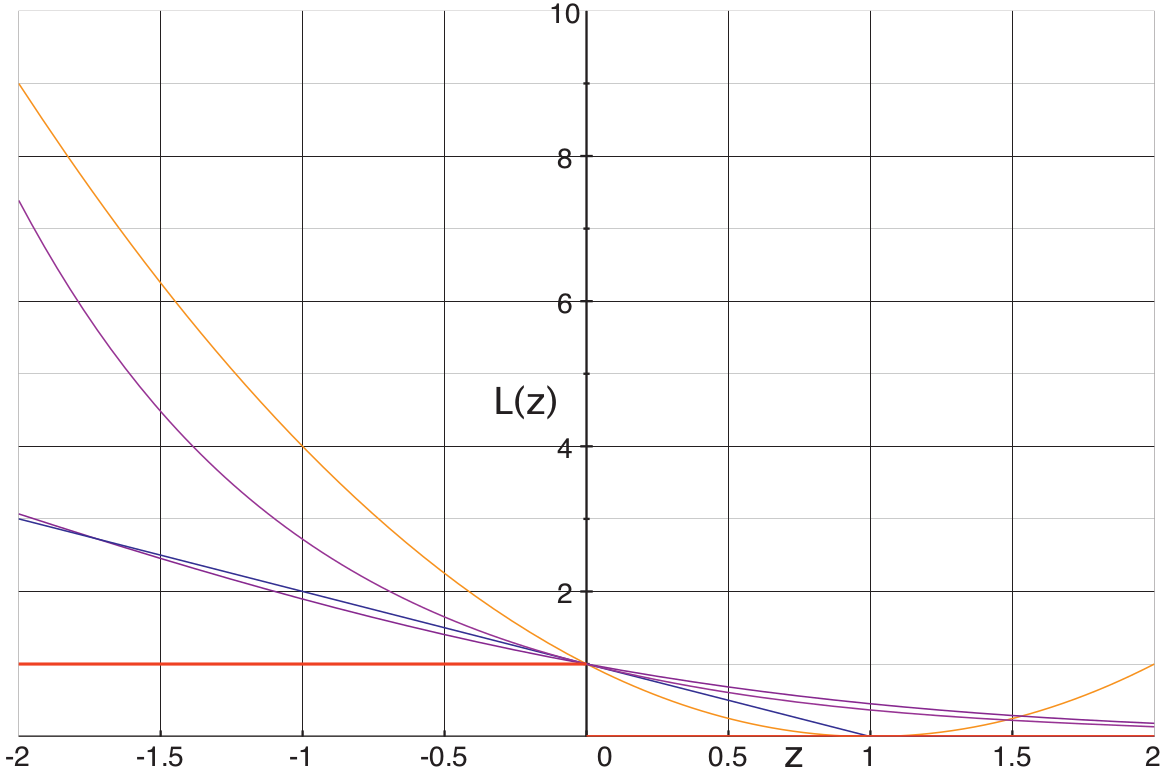
\includegraphics[width=60mm]{loss_functions.png}\\
\textbf{Loss functions:} from bottom-left $(i)$ 0-1 loss $L_{01}(z)=1$ if $z\leq 0$, and $L_{01}(z)=0$ if $z > 0$; $(ii)$ hinge loss $L_h(z)=(1 - z)$ if $z \leq 1$, and $L_h(z)=0$ if $z > 1$; $(iii)$ logistic loss $L_{log}(z) = log_2(1 + exp(-z))$; $(iv)$ exponential loss $L_{exp}(z) = exp(-z)$; $(v)$ squared loss $L_{sq}(z) = (1 - z)^2$ (this can be set to $0$ for $z > 1$, just like hinge loss).
\\
the loss function is often chosen to be \textbf{convex}, since optimizing a convex function is computationally more tractable
\\
\textbf{Ranking:} \textbullet Ranking error rate: $rank-err=\frac{err}{P+N}$, Ranking accuracy: $rank-acc=1-rank-err$
\subsection{Probability Estimation}
A class probability estimator is a scoring classifier that outputs probabilities over the k classes. A key issue here is that we generally do not have access to the true probabilities for training data.
\textbf{Empirical Probabilities:} \textbullet relative frequencies \textbullet $m-estimate=\frac{N_i+m\pi_i}{|S|+m}, \sum _{i}{\pi_i} $ \textbullet $Laplace\_correction=\frac{N_i+1}{|S|+k}$, $k$ is the number of classes
\end{document}
